\chapter{Introduction}
\label{chap:intro}
\typeout{START_CHAPTER "intro" \theabspage}

\section{Background}

% establish context
% crafted examples to fit data/problem e.g. CNNs, RNNs.
% generative modelling task, irregularly sampled data task, 

A central pattern in the advancement of deep learning is crafting methods and architectures for the task and data at hand. An image is structured in two dimensions, thus a two-dimensional convolutional kernel is a sensible modelling choice. Time series such as speech waveforms often have a causal relationship between past and future events, and recurrent neural networks share this property. Transformers build on this with parallel training computation over the sequence dimension and longer context modelling. These choices carefully consider the data, the form of the task, and scale required.

% whats wrong with conv, rnn, attention, depth not continuous, time not continuous, 

Typically, these models are constrained to discrete sequences of hidden layers. This constraint lacks support for modelling continuous dynamics, which may be more generalisable since a continuous process can be identical to a discrete process, but the reverse is not true. Recurrent nets may be applied to continuous time series, but they cannot model a continuous process. Overcoming these limitations has become a topic to be investigated.

Recent years have witnessed a growing academic interest in \textit{neural differential equations}. These models parametrise a vector-field with a neural network, enabling a continuous hidden state. The result has two key benefits for information processing: 1) \textbf{continuous-depth} allows scalable and adaptive models, and 2) alternatively the continuous dynamics can be tied to the continuity of the data: these \textbf{continuous-time} models can process streams of data that arrive at irregular times. The generalisations of these two claims to applied tasks are the focus of this thesis.

\paragraph{Pre-requisites} This thesis assumes familiarity with deep learning, differential equations, and speech technology.

% hidden state: prev see discrete sequence (jumps, highly constrained), network learning dynamics is good
% continuous depth: explain why its good, argue
% continuous time: 

\section{A brief review of neural differential equations}
% brief review
% CNFs, CDEs
\begin{figure}
    \centering
    \includegraphics[width=0.5\linewidth]{}
    \caption{Caption}
    \label{fig:placeholder}
\end{figure}
% focus on ODE, not the origin, one popular NN is resnet, this is like an ODE, not WHO, WHAT
% h_u+1 = ?. h_u = h_u + f(h). ...
The development of a deep learning model considers the definition of a successive hidden state
\[
\vh_{u+1} = \quad ?.
\]
A strong option is a residual layer
\[
\vh_{u+1} = \vh_u + \vf(\vh_u; \theta_u),
\]
which is the current hidden state plus the output of a learned neural network $\vf$, with trainable parameters $\theta_u$. This equation is similar to an Euler discretisation with step-size $\Delta u = 1$
\[
\vh_{u+1} = \vh_u + \vf(\vh_u; \theta_u)\cdot 1.
\]
Through this observation, $\vf$ becomes a \textit{vector field}. This vector field is variant to depth $u$ through specific parameters at each layer $\theta_u$, although a typical vector field would simply depend on depth $u$ directly. In addition to depending on $u$, another relaxation would be to support continuous $u$ and arbitrary step-size $\Delta u$, 
\[
\vh_{u+\Delta u} = \quad ?.
\]
The desired relaxations can be supported by a continuous Euler update
\[
\vh_{u+\Delta u} = \vh_u + \vf(\vh_u, u; \theta)\cdot \Delta u.
\]
This form of update with a parametrised vector field is known as a \textit{neural ordinary differential equation}. Formally, this leads to the definition of the hidden state as
\[
\vh_u = \vh_0 + \int_0^u\vf_\theta(\vh_s, s)\dd s.
\label{eq:cnf}
\]
A neural ODE is a flexible architecture that is easier to work with on certain tasks than non-continuous models. For example, a continuous-depth generative model can be constructed by bounding $u$ between 0 and $U$, then modelling a flow between a simple distribution at $u=U$ and a data distribution at $u=0$. This flow is optimised end-to-end by allocating a single set of parameters $\theta$ to support general $u$, rather than optimising a subset of the flow at discrete points. 

% 
This form of generative model is a \textit{continuous normalising flow}, and can be trained by maximum likelihood or a variational lower bound. There is much discussion on how to optimise a Neural ODE. A usual distinction is simulation vs simulation-free methods. Methods such as the continuous adjoint simulate the ODE forwards and backwards to compute gradient, whereas others construct a reference flow which can be sampled analytically and regressed. This thesis considers the many ways to optimise a simulation-free probabilistic flow e.g. diffusion, flow-matching. 


Another perspective considers the flexibility of continuously described dynamics, which is unsurprisingly useful for describing continuous dynamics. For example, the hidden state $\vh_u$ can be evaluated for any $u$, which allows the generation of irregularly sampled time-series e.g. $u\in\{1,3,4,6,7,11\}$. Examples of irregularly sampled data include medical data, stock market trading, and text labels aligned to speech recordings.






% explain difference between end-point and intermidiate states style of task, maybe diagrams

\section{Known vs unknown generalisations}
% section known generalisations vs unknown generalisations
% we care about likelihood, intermidiate optimisation, 
% speech support large LL, unlimited density, countably infinite, 
% dynamics of hidden state is a debate, should it have Brownian motion? 

Continuous normalising flows such as diffusion models have become strong models for TTS, but their probabilistic strength is unmeasured. Models such as Grad-TTS have scored higher in subjective evaluation, and they can alternatively be evaluated objectively by likelihood. The likelihood of the data determined by the model determines how important the probabilistic component is within the pipeline. The meaning of ``likelihood'' in a task such as TTS is naturally the likelihood of an acoustic observation given a text source. Models have not been evaluated this way which leads to a gap in research.

Continuous normalising flows have become strong models for DNS, but whether designs that better fit the nature of the task are better is unknown. Diffusion models form a flow between standard normal source and a target data distribution by simulating reverse Brownian motion. Schr\"odinger bridges alternatively support a data source, but maintain the assumption that the flow should be Brownian. It is uncertain to what extent Brownian motion is necessary for high-quality DNS.

Continuous-time models have been used for speech tasks with end-point optimisation ($\vh_U$), but tasks such as TTS and ASR optimise intermediate states $\vh_u$. An additional complication is the coupling of a continuous speech signal and a discrete sequence of tokens. This outlines a gap in the known generalisations of continuous-time models applied to speech tasks.



\section{Research questions}
% identify problem
% aims, RQs, hypothesis
\subsection{Continuous-depth}
There is little to no detailed investigation into the generalisations of NDEs on speech processing tasks such as speech synthesis, recognition, and noise suppression. Although breakthrough implementations of CNFs for speech processing exist, there is a lack of studies investigating the likelihood of these models. Furthermore, no previous study has analysed the impact of Brownian motion in noise suppression, a task that modifies the typical Gaussian-to-data formula to data-to-data. This forms two research questions.

% why add noise to a noise removal task?
% don't use data-to-data term

\paragraph{RQ1}
How well does diffusion model likelihood correspond to expected behaviour in image and speech synthesis?

Diffusion models are an efficient way to train CNFs (\eqref{eq:cde}), and have been used for image and speech synthesis. How probabilistic is our model in this case? What are the semantics of ``likelihood'' in these contexts? Does a picture of a red ball with caption ``blue cube'' have a low likelihood? Does a spoken utterance and its transcript have a high likelihood?

\paragraph{RQ2}
How well do CNFs generalise to data-to-data tasks such as deep noise suppression, and how important is Brownian motion?

DNS deals with transforming a noise-speech mixture into a clean speech signal. Diffusion models exploit Brownian motion to learn this function. How necessary is Brownian motion? Flow matching is an alternative method that supports data-to-data transformations without Brownian motion, how well does this fit to the DNS task?

\subsection{Continuous-time}
% mention studies that have been made, 

\paragraph{RQ3}
% duration question, it is important, tasks where intermidiate state is important
% is inter observation process useful?
What role can neural CDEs play in speech synthesis?

Is modelling irregularly sampled time-series useful for describing text-speech alignment? Is the propagation of duration information useful? What aspects of the design space of rough path theory affect synthesis quality? Do CDEs allow better synthesis control?


\paragraph{RQ4}
How much memory requirement can be reduced when using continuous-time backpropogation for non-endpoint optimisation of neural ODEs?

Does a neural ODE require less parameters? Is the model quality the same? Does it take longer to train than gradient check-pointing or recurrent modules with backpropogation through time? 

\section{Contributions}
% design and methods
% value

Chapter X answers RQ1 with an empirical investigation into how likelihood is computed on different data setups. It is shown that less accurate transcriptions have higher likelihood. For image synthesis, images with correct captions did not have a higher likelihood than those with incorrect captions.

Chapter X answers RQ2 by constructing a flow matching speech denoiser and comparing it with a Schr\"odinger bridge model. Schr\"odinger bridges can be thought of as a data-to-data CNF whose intermediate state moves with Brownian motion, whereas flow matching has a linear interpolating state. Experiments show little evidence motivating Brownian motion. Additional inference schemes are tested, where it is suggested that once a flow matching model is trained, it is better to directly predict the data from the model rather than solve an ODE.

Chapter X forms RQ3 through emotional TTS. It is found that human judgment to the intended emotion style is better correlated with a continuous-time mechanism in place.

Chapter X answers RQ4 by training NDE decoders on top of pretrained ASR models, or learning in an end-to-end manner.

\section{Dissertation outline}
% structure overview
\begin{figure}
    \centering
    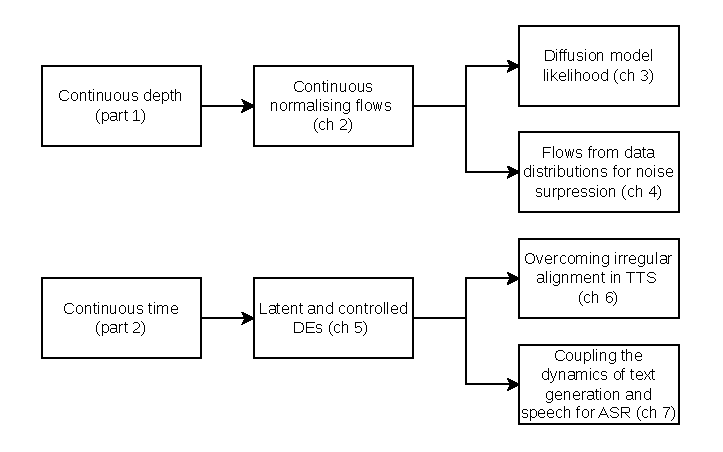
\includegraphics[width=\linewidth]{plots/thesis_contents.drawio.pdf}
    \caption{Enter Caption}
    \label{fig:placeholder}
\end{figure}
The rest of this dissertation is organised into two parts. The first part is concerned with CNFs, which studies continuous-depth models for speech and image data. Chapter X provides a background on training CNFs with diffusion, and how this can be used for speech and image synthesis. Chapter X examines the empirical properties of diffusion likelihood. Chapter X builds further on CNFs by reviewing methods for data-to-data processes with Schr\"odinger bridge and flow matching models. These models are then used to explore the path design in continuous depth speech denoisers by observing the use of Brownian motion in chapter X. The second part considers continuous-time models for speech synthesis and recognition. Chapter X introduces a background to neural CDE's, which allow a neural ODE to react to an input stream of data. Neural CDE's are then used in chapter X and X for the aforementioned tasks. Concluding remarks to the new point of view found in this thesis are given in chapter X.

\section{Publications}